%%%%%%%%%%%%%%%%%%%%%%%%%%%%%%%%%%%%%%%%%%%%%%%%%%%%%%%%%%%%%%%%%%%%%%%%%%%%%%%
%% Descr:       Vorlage für Berichte der DHBW-Karlsruhe
%% Author:      Prof. Dr. Jürgen Vollmer, vollmer@dhbw-karlsruhe.de
%% $Id: bericht.tex,v 1.19 2016/03/16 16:59:41 vollmer Exp $
%%  -*- coding: utf-8 -*-
%%%%%%%%%%%%%%%%%%%%%%%%%%%%%%%%%%%%%%%%%%%%%%%%%%%%%%%%%%%%%%%%%%%%%%%%%%%%%%%

\documentclass[
   ngerman          % neue deutsche Rechtschreibung
  ,a4paper          % Papiergrösse
% ,twoside          % Zweiseitiger Druck (rechts/links)
% ,10pt             % Schriftgrösse
  ,11pt
% ,12pt
  ,pdftex
%  ,disable         % Todo-Markierungen auschalten
]{report}

% Bitte die Codierung Ihrer Dateien auswählen:
% \usepackage[latin1]{inputenc}    % Für UNIX mit ISO-LATIN-codierten Dateien
% \usepackage[applemac]{inputenc}  % Für Apple Mac
% \usepackage[ansinew]{inputenc}   % Für Microsoft Windows
\usepackage[utf8]{inputenc}        % UTF-8 codierte Dateien
                                   % Dieses Dokument ist unter Unix erstellt, daher
                                   % wird diese Input-Codierung benutzt.

\usepackage{bericht}

%%%%%%%%%%%%%%%%%%%%%%%%%%%%%%%%%%%%%%%%%%%%%%%%%%%%%%%%%%%%%%%%%%%%%%%%%%%%%%%
%% Angaben zur Arbeit
%%%%%%%%%%%%%%%%%%%%%%%%%%%%%%%%%%%%%%%%%%%%%%%%%%%%%%%%%%%%%%%%%%%%%%%%%%%%%%%

\newcommand{\Autor}{Dominik Klysch}
\newcommand{\MatrikelNummer}{1010579}
\newcommand{\Kursbezeichnung}{TINF18B4}

\newcommand{\FirmenName}{N/A}
\newcommand{\FirmenStadt}{N/A}
% \newcommand{\FirmenLogoDeckblatt}{\includegraphics[width=3cm]{TODO}}

% Falls es kein Firmenlogo gibt:
\newcommand{\FirmenLogoDeckblatt}{}

\newcommand{\BetreuerFirma}{TODO}
\newcommand{\BetreuerDHBW}{TODO}

%%%%%%%%%%%%%%%%%%%%%%%%%%%%%%%%%%%%%%%%%%%%%%%%%%%%%%%%%%%%%%%%%%%%%%%%%%%%%%%%%%%%%

\newcommand{\Was}{Programmentwurf}
% Wird auf dem Deckblatt in der Erklärung benutzt

%%%%%%%%%%%%%%%%%%%%%%%%%%%%%%%%%%%%%%%%%%%%%%%%%%%%%%%%%%%%%%%%%%%%%%%%%%%%%%%%%%%%%

\newcommand{\Titel}{Advanced Software Engineering}
\newcommand{\AbgabeDatum}{TODO}

\newcommand{\Dauer}{X Wochen}

%\newcommand{\Abschluss}{Bachelor of Engineering}
\newcommand{\Abschluss}{Bachelor of Science}

%\newcommand{\Studiengang}{Informationstechnik}
\newcommand{\Studiengang}{Angewandte Informatik}

\hypersetup{%%
  pdfauthor={\Autor},
  pdftitle={\Titel},
  pdfsubject={\Was}
}

%%%%%%%%%%%%%%%%%%%%%%%%%%%%%%%%%%%%%%%%%%%%%%%%%%%%%%%%%%%%%%%%%%%%%%%%%%%%%%%

% Wenn \includeonly{..} benutzt wird, werden nur diese Kaptitel ausgegeben.
\includeonly{
  abk
  ,0_einleitung
  ,1_kapitel
  ,2_kapitel
  ,3_kapitel
  ,4_kapitel
  ,5_kapitel
  ,6_kapitel
  ,7_kapitel
  ,8_kapitel
}

%%%%%%%%%%%%%%%%%%%%%%%%%%%%%%%%%%%%%%%%%%%%%%%%%%%%%%%%%%%%%%%%%%%%%%%%%%%%%%%

% Benutzt man das "biblatex"-Paket, dann muß das hier stehen:
% siehe auch die mit BIBLATEX markierten Zeilen in bericht.sty
\bibliography{bericht}
\newcounter{savepage}
\begin{document}

%%%%%%%%%%%%%%%%%%%%%%%%%%%%%%%%%%%%%%%%%%%%%%%%%%%%%%%%%%%%%%%%%%%%%%%%%%%%%%%

\pagenumbering{roman}
\begin{titlepage}
  \begin{center}
    \vspace*{-2cm}
    \FirmenLogoDeckblatt\hfill\includegraphics[width=4cm]{dhbw-logo}\\[2cm]
    {\Huge \Titel}\\[2cm]
    {\Huge\scshape \Was}\\[2cm]
    {\large für die Prüfung zum}\\[0.5cm]
    {\Large \Abschluss}\\[0.5cm]
    {\large des Studienganges \Studiengang}\\[0.5cm]
    {\large an der}\\[0.5cm]
    {\large Dualen Hochschule Baden-Württemberg Karlsruhe}\\[0.5cm]
    {\large von}\\[0.5cm]
    {\large\bfseries \Autor}\\[1cm]
    {\large Abgabedatum \AbgabeDatum}
    \vfill
  \end{center}
  \begin{tabular}{l@{\hspace{2cm}}l}
    Matrikelnummer & \MatrikelNummer  \\
    Kurs           & \Kursbezeichnung \\
  \end{tabular}
\end{titlepage}

%%%%%%%%%%%%%%%%%%%%%%%%%%%%%%%%%%%%%%%%%%%%%%%%%%%%%%%%%%%%%%%%%%%%%%%%%%%%%%%

% Nur für Bachelorarbeiten einfügen:
\tableofcontents           % Inhaltsverzeichnis hier ausgeben

% Jetzt kommt der "eigentliche" Text
\setcounter{savepage}{\arabic{page}}
\pagenumbering{arabic}
%% TODO Einleitung / Erklärung auch dass UI nur Optional ist um Funktion anzuschauen
%% TODO Rechtschreibung prüfen
\chapter{Einleitung}

In diesem Programmentwurf wurde ein User Verwaltungs System Backend für einen beliebigen Game Server entworfen.
Das bedeutet dieses System soll auf die Datenbank eines Game Servers mit Usern zugreifen und diese über eine API Schnittstelle verwalten.
Es wurde auch ein simples UI entworfen um die Funktionalität der API Schnittstelle einfacher überprüfen zu können.
Dieses UI gehört aber nicht zum eigentlichen Programmentwurf und sollte daher als von der Bewertung ausgeschlossen betrachtet werden.

\section{Installation}

\subsection{Requirements}

Benötigte Software zum ausführen des Programmentwurfs:

\begin{itemize}
    \item Java 11
    \item Docker Desktop
    \item docker-compose
\end{itemize}

\subsection{Starten der Anwendung}
Befehle im root Order der Repo ausführen.
Das erste bauen könnte etwas länger dauern.

Bauen und ausführen: docker-compose up --build
\newline
Starten ohne neu bauen: docker-compose start
\newline
Stoppen: docker-compose stop
\newline
Stoppen + alles löschen: docker-compose down --volumes
\newline

Nach dem starten sollte gewartet werden bis in der Console der Datenbank steht: mysqld: ready for connections.



Default Admin User: email: root@example.com pw: example




Frontent: http://localhost:3000/
Wenn noch keine Reports / Bans in der DB sind zeigt das UI dauerhaft einen Ladebalken auf diesen Seiten an.
Wenn ein User einen neuen Rang bekommt, aber noch im UI angemeldet ist: Einmal neu im UI Anmelden damit eine neue Session mit dem aktuellen Rang ausgestellt wird.
\newline
API-Server: http://localhost:7001/
\newline
Datenbank: localhost:3306



\subsection{Ausführen der Tests}

Befehl im root Order des Backends ausführen: ./gameserver-backend

Wichtig die Mockito version benötigt Java 11 !

Befehl zum ausführen der Unit tests: mvn test
\chapter{Domain Driven Design}
\section{Analyse der Ubiquitous Language}

%% „allgegenwärtige Sprache“
%% Gleiche Begriffe in Domäne und Sourcecode
%% Jede Domäne besitzt eine eigene Fachsprache
%% Verstehen, warum diese Fachsprache gesprochen wird
%% Nicht versuchen, diese Fachsprache in „eigene“ Begriffe zu übersetzen
%% Ubiquitous Language bezeichnet die von Domänenexperten und Entwicklern gemeinsam im Projekt verwendete Sprache

%% Die Ubiquitous Language soll die Kluft reduzieren, indem Domänenexperten und Entwickler eine gemeinsame Sprache finden, die
%% - Alle relevanten Konzepte, Prozesse und Regeln der Domäne beschreibt
%% - Zusammenhänge verdeutlicht
%% - Mehrdeutigkeiten und Unklarheiten beseitigt

\begin{center}
    \begin{tabular}{ | l | l | }
        \hline
        Wort & Bedeutung                   \\ \hline
        Test & Test ist sehr toll          \\ \hline
        User & User spielen auf dem Server \\
        \hline
    \end{tabular}
\end{center}


\section{Analyse und Begründung der verwendeten Muster}

\subsection{Value Objects}

%% Value Objects (VO) sind einfache Objekte ohne eigene Identität
%% VO sind unveränderlich (immutable)
%% Ein VO kapselt ein „Wertkonzept“ und wird nur durch seine Eigenschaften oder Werte beschrieben -> daher: Value Object
%% Daraus folgt: zwei VO sind gleich, wenn sie die selben Werte haben

%% Vorteile von Unveränderlichkeit
%% Wenn ein Objekt gültig konstruiert wurde, kann es danach nicht ungültig werden
%% ->Einhalten von Invarianten der Domäne im Code wird sehr einfach
%% Unveränderliche Objekte sind frei von Seiteneffekten
%% -> Code ist weniger anfällig für ungewolltes Verhalten

%% Vorteile von Value Objects
%% Verbessern die Deutlichkeit und Verständlichkeit durch Modellierung von fachlichen Domänenkonzepten
%% Kapseln Verhalten und Regeln
%% Unveränderlich (frei von Seiteneffekten , beispielsweise Aliasing)
%% Selbst-Validierend
%% Leicht testbar

%% Implementierung von Value Objects in Java
%% lasse ist „final“ deklariert (Vererbung unterdrücken)
%% Alle Felder sind „blank final“ deklariert
%% equals() und hashCode() sind passend überschrieben
%% Ist nach Konstruktion in gültigem Zustand (andernfalls muss Konstruktion fehlschlagen)
%% Keine Setter oder andere Methoden, durch die Felder geändert werden können
%% Alle Methoden mit Rückgabewert liefern entweder:
%% Unveränderliche Rückgabewerte (immutable) oder
%% Defensive Kopien


\subsection{Entities}

%% Eine Entity unterscheidet sich in drei wesentlichen Punkten von einem VO:
%% Sie hat eine eindeutige ID innerhalb der Domäne
%% Zwei Entities sind verschieden, wenn sie verschiedene IDs haben; ihre Eigenschaften sind unerheblich
%% Eine Entity hat einen Lebenszyklus und verändert sich während ihrer Lebenszeit
%% Wie auch VO sollen Entities die Einhaltung der für sie geltenden Domänenregeln (Invarianten) forcieren:
%% Es darf nicht möglich sein, eine Entity mit ungültigen Werten zu erzeugen
%% Es darf nicht möglich sein, eine Entity nach Konstruktion in einen ungültigen Zustand zu versetzen
%% Entities sollten so viel Verhalten wie möglich in VO auslagern
%% (mindestens) die öffentlichen Methoden einer Entity sollten Verhalten beschreiben und nicht nur einfache getter/setter darstellen

%% Strategien für einzigartige Identitäten
%% Es gibt mehrere Strategien, um eine Entity eindeutig identifizierbar zu machen
%% Jede Strategie hat mehr oder weniger ausgeprägte Vorteile und Nachteile
%% Die jeweils passende Strategie hängt (wie immer) von den Anforderungen ab
%% Es spricht nichts dagegen, mehrere Strategien in einer Anwendung zu verwenden
%% Grundsätzliche Unterscheidung: 
%% natürliche Schlüssel und Surrogatschlüssel


%% Value Objects vs Entities
%% http://prntscr.com/w4mgu2



\subsection{Aggregates}

%% Wenn die Domäne maßstabsgetreu modelliert wird, findet man viele Entities und VO, die große Objektgraphen mit oft bidirektionalen Abhängig-keiten bilden
%% Das wird schnell ungemütlich:
%% Wahrscheinlichkeit nicht eingehaltener Regeln steigt
%% Verstärkt Kollisionen beim gleichzeitigen Bearbeiten
%% Performance-Einbußen durch Warten auf Sperrenfreigabe
%% Lange Wartezeiten beim Laden und Speichern
%% Aggregate gruppieren die Entities und VO zu gemeinsam verwalteten Einheiten
%% Jede Entity gehört zu einem Aggregat – selbst wenn das Aggregat nur aus dieser Entity besteht
%% Aggregate reduzieren die Komplexität der Beziehungen zwischen den Objekten
%% Das Aggregat wird immer als Einheit betrachtet und verwaltet (geladen und gespeichert)
%% Es gibt klare Regeln, wie außenstehende Objekte mit dem Aggregat interagieren dürfen
%% In jedem Aggregat übernimmt eine Entity die Rolle der Aggregate Root Entity bzw. des Aggregat Root (AR)
%% Alle Zugriffe auf das Aggregat müssen über das AR erfolgen
%% Auch Zugriffe auf die inneren Elemente des Aggregat
%% Langfristige direkte Referenzen auf innere Elemente sind nicht erlaubt
%% Nur temporäre Referenzen während einer Berechnung
%% Eines pro Aggregat
%% Das AR kann als eine Art 
%% „Türsteher“ alle Zugriffe auf 
%% das Aggregat kontrollieren
%% Zentrale Stelle zur Über-
%% wachung der Domänenregeln
%% Beispiel: Der Gesamtpreis einer Erstbestellung darf nicht mehr als 100 € betragen
%% aggregatsinterne Angelegenheiten bleiben „in der Familie“
%% Zugriff auf Aggregat nur über Aggregate Root
%% Wenn das AR Referenzen auf innere Objekte herausgeben muss, sollten das immer defensive Kopien oder Immutable-Dekorierer sein
%% Aussenwelt muss eine Methode auf dem AR aufrufen, wenn der innere Zustand des AR verändert werden soll
%% Das Aggregat sorgt dafür, dass sein Zustand immer den Domänenregeln entspricht
%% Alle Änderungen gehen über den AR und sind daher bekannt
%% Wenn die Außenwelt den AR „vergisst“, ist das gesamte Aggregat nicht mehr erreichbar

%% Zusammenfassung Aggregate
%% Aggregate sind Zusammenfassungen von Entities und Value Objects
%% Jedes Aggregat bildet eine eigene Einheit (auch für Create, Read, Update, Delete – CRUD)
%% Wird immer vollständig geladen und gespeichert
%% Aggregate
%% entkoppeln die Objektbeziehungen
%% bilden natürliche Transaktionsgrenzen
%% sichern Entity-/VO-übergreifende Domänenregeln zu
%% Aggregate sind mächtig, aber auch schwierig


\subsection{Repositories}

%% Kapseln die Logik für das Persistieren und Erzeugen von Entities, Value Objects und Aggregates
%% Halten das Modell frei von „accidental complexity“
%% Repositories vermitteln zwischen der Domäne und dem Datenmodell
%% Sie stellen der Domäne Methoden bereit, um Aggregates aus dem Persistenzspeicher zu lesen, zu speichern und zu löschen
%% Der konkrete technische Zugriff (accidental complecity) auf den Speicher (relationale DB, NoSQL, XML-Dateien usw.) wird vom Repository verborgen
%% Dadurch bleibt die Domäne von technischen Details unbeeinflusst
%% Repositories arbeiten direkt mit Aggregates zusammen
%% je Aggregate existiert also typischerweise ein Repository
%% Repositories liefern immer die Aggregate Roots (und damit den Zugriff auf den Rest) zurück
%% Die Definition der Repositories ist Teil des Domain Code
%% Die Implementierung findet „außerhalb“ statt
%% Die Methoden des Repository-Interface werden in der Sprache der Domäne benannt
%% Der Klassenname kann „Pure Fabrication“ sein
%% Der Rest der Anwendung muss eine bestimmte Aggregate Root anhand ihrer Eigenschaften finden können
%% Diese Abfragen sind die wichtigste Aufgabe des Repositories
%% Die Abfragen sollten genau zu den Aufgaben der Domäne passen
%% Selbst wenn es eine allgemeine Abfrage (über Kriterien) gibt, lohnen sich die speziellen Methoden
%% Das Repository kann für die Erstellung von Identifikationen (IDs) für neue Root Entities zuständig sein
%% Kann zusätzliche speicherseitige Prüffelder bei Veränderungen setzen („zuletztGeändertAm“)
%% Kann für Unit Tests leicht gemockt werden
%% Kann für Integrationstests ohne Datenbank durch eine In-Memory-Implementierung ersetzt werden
%% Die Implementierung erfolgt normalerweise in einer technischen Schicht der Anwendung (DB, Infrastruktur, …) und nicht innerhalb des Domänenmodells
%% Keine Vermischung von essential und accidental complexity

%% Zusammenfassung Repositories
%% Repositories bieten dem Domain Code Zugriff auf persistenten Speicher
%% In der Granularität von Aggregates
%% Direkter Zugriff immer nur auf die Aggregate Roots
%% Repositories verbergen die konkrete Speicher- technologie vollständig vor dem Domain Code
%% Anti-Corruption-Layer zur Persistenzschicht
%% Repositories bieten passend für die Domäne Abfragemöglichkeiten auf den Datenbestand
%% Adapter zwischen Anwendung und Datenbank


%% Factories 
%% Factories haben nur einen einzigen Zweck:
%% das Erzeugen von Objekten
%% Factories sind ein allgemein nützliches Konzept, unabhängig von DDD
%% Wenn die Logik für das Erzeugen einer Entity, eines Aggregates oder eines VO komplex wird, kann dies den eigentlichen Zweck des Objekts verschleiern (Verletzung des Single-Responsibility-Prinzips)
%% Factories helfen, indem sie dem Objekt die Verantwortung für seine Konstruktion abnehmen; dadurch kann sich das Objekt auf sein Verhalten konzentrieren
%% Der Begriff „Factory“ wird in OOP mehrdeutig verwendet. Es bezeichnet sowohl:
%% Das allgemeine Konzept einer Factory:
%% irgendein Objekt oder irgendeine Methode zur Erzeugung andere Objekte als Konstruktor-Ersatz
%% spezielle Erzeugungs-Muster
%% Factory Method
%% Abstract Factory
%% Im DDD meint man mit Factory normalerweise das „allgemeine Konzept“
%% Allgemein ist eine Factory irgendein Objekt/ irgendeine Methode als Konstruktor-Ersatz (siehe unten)




\subsection{Domain Services}

%% Ein Domain Service hat zwei Haupt-Einsatzzwecke:
%% Abbildung von komplexem Verhalten, Prozessen oder Regeln der Problemdomäne, die nicht in eindeutig einer bestimmten Entity oder einem bestimmten VO zugeordnet werden können
%% Definition eines „Erfüllungs-Vertrages“ für externe Dienste, damit das Domänenmodell nicht mit unnötiger „accidental complexity“ belastet wird
%% Manchmal kann ein bestimmtes Verhalten oder eine bestimmte Regel nicht eindeutig einer Entity oder einem VO zugeordnet werden
%% Beispiel:
%% Berechnung der Zahlungsmoral eines Kunden
%% Benötigt Kunde
%% Benötigt Rechnungen
%% Benötigt Kontenbewegungen
%% Die Domäne kann zur Erfüllung der Anforderungen auf externe Unterstützung angewiesen sein, beispielsweise durch einen Webservice, der von einer Fremdanwendung bereitgestellt wird
%% Innerhalb des Domänenmodells kann dazu ein Domain Service als Vertrag (Interface) definiert werden
%% Außerhalb des Domänemodells kann  dann ein „Dienstleister“ (beispielsweise in der Infrastruktur-Schicht – siehe Onion Architecture) diesen Vertrag implementieren und die benötigten Funktionen bereitstellen 
%% urch die Definition eines Vertrages kann das Domänenmodell vorgeben, was für ein Ergebnis erwartet wird („CreditWorthiness „) und welche Daten es zur Erfüllung des Vertrages bereitstellt („Customer“)
%% „fachlich“ ist dann alles relevante im Domänenmodell abgebildet – lediglich die technischen Details werden an eine Schicht außerhalb des Domänenmodells delegiert
%% Der Domain Service bezieht sich auf ein Domänenkonzept, das nicht natürlicherweise Teil einer Entity oder eines Value Object ist
%% Die Schnittstelle (die Methodensignaturen) verwendet die Begriffe des Domänenmodells
%% Ein- und Ausgabeparameter sind Entities und VO
%% Der Domain Service selbst ist zustandlos
%% Jede konkrete Instanz des Domain Service kann verwendet werden (alt oder neu)
%% Er darf aber (global sichtbare) Seiteneffekte haben









%% Zusammenfassung

%% Um die Entities und Value Objects technisch sauber implementieren zu können, benötigen wir unterstützende Strukturen
%% Domain Services enthalten Use Cases oder entkoppeln von Drittsystemen
%% Aggregates gruppieren Entities und vereinfachen die Beziehungen zwischen den Gruppen
%% Aggregate Roots stellen die primären Objekte dar
%% Repositories entkoppeln die Persistenz und machen die Aggregate Roots einfach auffindbar
%% Factories erzeugen Objektgraphen mit komplexen Konstruktionsregeln und entlasten den Konstruktor (Einhaltung Single Responsibility Principle)


\chapter{Clean Architecture}

%% Plugins (DB / GUI) -> Adapters (Presenters, Controllers, Gateways) -> Application Code (Use Cases) -> Domain Code (Entities) -> Abstraction Code (Generic Entities (mathematische Konzepte))
%% Abstraction Code: 
%%  Mathematische Konzepte (z.B. Matrizen)
%%  Algorithmen und Datenstrukturen (z.B. Zelluläre Automaten)
%%  Abstrahierte Muster (z.B. Quantitäten)
%%  !!!!!Häufig nicht notwendig!!!!
%% 
%% Domain Code:
%%  Entities 
%%  Implementiert organisationsweit gültige Geschäftslogik
%%  Sollte sich am seltensten ändern
%% 
%% Application Code:
%%  Use Cases
%%  Implementiert die anwendungsspezifische Geschäftslogik
%%  Steuert den Fluss der Daten und Aktionen von und zu den Entities
%% 
%% Adapters:
%%  Diese Schicht vermittelt Aufrufe und Daten an die inneren Schichten
%%  Formatkonvertierungen
%%  Oftmals nur einfache Datenstrukturen, die hin- und hergereicht werden
%%  Anti-Corruption Layer
%% 
%% Plugins:
%%  Diese Schicht greift grundsätzlich nur auf die Adapter zu
%%  Enthält Frameworks, Datentransportmittel und andere Werkzeuge (Datenbank, API)
%%  Wir versuchen, hier möglichst wenig Code zu schreiben
%%  Hauptsächlich Delegationscode, der an die Adapter weiterleitet
%% 
%% Grundregeln der Clean Architecture
%%  ● Der Anwendungs- und Domaincode ist frei von Abhängigkeiten
%%  ● Sämtlicher Code kann eigenständig verändert werden
%%  ● Sämtlicher Code kann unabhängig von Infrastruktur kompiliert und ausgeführt werden
%%  ● Innere Schichten definieren Interfaces, äußere Schichten implementieren diese
%%  ● Die äußeren Schichten koppeln sich an die inneren Schichten (Richtung Zentrum)

%% Konkrete Umsetzung
%% ●Nicht alle Klassenin einem Projekt
%% ●Schichtenbildung überPackages ist in Ordnung
%% ●Aber: keine Überprüfungdurch den Compiler
%% ●Lieber mehrere Projekte(„Multi-Projekt“)
%% ●Compiler findet nur Klassen–im eigenen Projekt–in referenzierten Projekten
%% Maven parent Pom

%% Ziel der Clean Architecture
%% Das Ziel der Clean Architecture ist, Code nur von langlebigerem Code abhängig zu machen
%% Wenn sich Technologien ändern müssen, kann die Anwendung unverändert bleiben

\section{Schichtarchitektur planen und begründen}

\begin{figure}[htbp]
    \centering
    \fbox{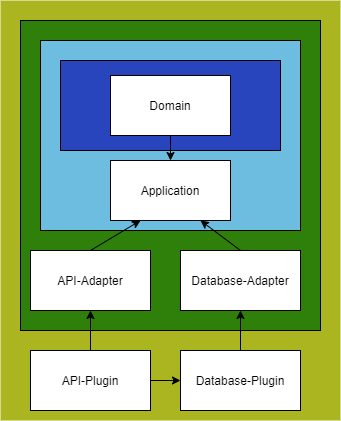
\includegraphics[width=6cm]{schichtarchitektur}}
    \caption{\label{flutter-1} Schichtarchitektur}
\end{figure}
%% genauer erklären warum es aufgespalten wurde!!!!
Die Schichtarchitektur ist in vier Schichten unterteilt: Plugin, Adapter, Application, Domain.
Die Plugin-Schicht wurde nochmals in API und Datenbank aufgeteilt um die übersichtlichkeit etwas zu erhöhen.
Dementsprechend wurde die Adapter-Schicht auch in API und Datenbank aufgeteilt und konvertiert die jeweiligen Objekt-Formate in die Formate der inneren Schichten.
Die Adapter rufen dann Funktionen aus der Application Schicht auf.
In der Application-Schicht liegt dann die eigentliche Logik der Anwendung und hier werden API und Datenbank zusammen geführt.
In der Domain Schicht befinden sich die Entities und Value Objects der Application Schicht,
dies dient dem Ziel diese in Zukunft in weiteren Application-Schichten einheitlich verwenden zu können.
Zusätzlich enthält die Domain Schicht die Repository-Interfaces welche von darunter liegenden Schichten implementiert werden um eine Inversion of Control zu erzeugen.
%% fundamental: von aussen nach innen!!!!!!!
%% TODO vlt bisschen mehr schreiben, Begründung fehlt
%% Anwendung macht xy
%% ich ordne folgende funktionen der folgenden Schicht zu ...
%% die sind da weil ...
%% Folgende schichten wurden nicht verwendet weil....
\chapter{Programming Principles}
\section{Analyse und Begründung für SOLID}
%% 
%% Single Responsibility Principle
%%  - Eine Klasse sollte nur eine Ursache oder einen Grund haben sich zu ändern
%%  - Niedrige Komplexität und Kopplung
%%  - Jede Klasse sollte nur eine Zuständigkeit haben
%%  - Eine Klasse erhält eine klar definierte Aufgabe
%%  - Komplexeres Verhalten entsteht durch Kombination mehrerer Objekte
%%  - Eine Klasse enthält Achsen auf der sich Anforderungen ändern können
%%  - Jede Zuständigkeit fügt eine weitere Achse hinzu
%%  - Jede Klasse sollte nur eine Achse haben

\subsection{Single Responsibility Principle}
Das Single Responsibility Principle sagt aus, dass eine Klasse nur eine Zuständigkeit haben sollte.
Somit hat jede Klasse eine klar definierte Aufgabe und es entsteht eine niedrige Komplexität des Codes.
Und um so niedriger die Komplexität des Codes desto besser lässt er sich warten und erweitern.

%% Open Closed Principle
%%  - Elemente der Software wie Klassen, Module, Funktionen sollten:
%%      - offen für Erweiterungen
%%      - geschlossen für Änderungen 
%%  - Erweiterungen durch Vererbung bzw.Implementierung von Interfaces
%%  - Neue Unterklasse mit angepasstem Verhaltenergänzen
%%  - Bestehender Code wird nicht geändert
%%  - Abstraktionen fördern die Erweiterbarkeit
%%  - Software ist nie immun gegen Änderungen
%%  - Der Entwickler entscheidet 
%%      - welche Erweiterungen möglich sind
%%      - was durch Änderungen ergänzt werden soll
%%  - Stabilität einer Klasse ist ausschlaggebend

\subsection{Open Closed Principle}
Durch das Open Closed Principle wird die Software offen für Erweiterungen aber geschlossen für Änderungen.
Das bedeutet der Code wird nur durch Vererbung bzw. Implementierung von Interfaces erweitert.
Dies führt dazu das bestehender Code nicht geändert wird, wodurch die Anwendung für eine gute kompatibilität über die Versionen sorgt.
Hierbei ist es wichtig viele Abstraktionen zu nutzen um die Erweiterbarkeit zu fördern.

%% Liskov Substitution Principle
%%  - Objekte eines abgeleiteten Typs müssen als Ersatz für Instanzen ihres Basistyps funktionieren ohne die Korrektheit des Programms zu ändern
%%  - Starke Einschränkung der Ableitungsregeln
%%  - Führt zur Einhaltung von Invarianzen
%%  - Invarianzen von Klassen berücksichtigen:
%%      - Abgeleitete Typen müssen schwächere Vorbedingungen haben
%%      - Abgeleitete Typen müssen stärkere Nachbedingungen haben
%%  - Design by Contract kann helfen Verstöße zufinden
%%  - Ableitung in OOP ist mehr eine "verhält sich wie" Beziehung anstatt einer "ist ein" Beziehung

\subsection{Liskov Substitution Principle}
Im Liskov Substitution Principle werden Ableitungsregeln stark eingeschränkt was zu einer Einhaltung von Invarianzen führt.
Hierbei müssen abgeleitete Typen schwächere Vorbedingungen und stärkere Nachbedingungen haben.
Durch dieses Prinzip ergeben sich somit im OOP \glqq verhält sich wie\grqq{} Beziehungen statt den üblichen \glqq ist ein\grqq{} Beziehungen.
Somit kann man sich auf ein bestimmtes Verhalten der abgeleiteten Typen verlassen, wenn man das Verhalten des Basistyps kennt.

%% Interface Segregation Principle
%%  - Anwender sollten nicht von Funktionen abhängig sein, die sie nicht nutzen
%%  - Schwere(fat) Interfaces und Klassen bündelnviel Funktionalität:
%%      - Ein Anwender einer Methode eines Interfaces istautomatisch abhängig von Änderungen ananderen Methoden des Interfaces
%%      - Ein Anwender hat Zugriff auf Methoden, die nichtfür ihn bestimmt sind
%%  - Interfaces passend zu den Anwenderngestalten
%%  - Führt dazu, dass Typen meist mehrere Interfaces implementieren
%%  - Ein Typ bedient dadurch mehrere Anwender
%%  - Schwere Klassen können nach wie vorbestehen, aber Anwender ist nur von leichten Interfaces abhängig
\subsection{Interface Segregation Principle}
Das Interface Segregation Principle sorgt dafür, dass Anwender nicht von Funktionen abhängig sind die sie gar nicht nutzen.
Dies wird ermöglicht indem man statt einzelnen großen schweren Interfaces mit vielen Funktionen, viele kleine leichte Interfaces mit wenigen Funktionen implementiert.
Somit kann man seine Klasse passend für den Anwendungszweck anpassen ohne unnötige extrafunktionen mit zu schleppen.

%% Dependency Inversion Principle
%%  - Klassischerweise sind High-Level Module von Low-Level Modulen abhängig:
%%      - Änderung in einer Low-Level Implementierungführt zu Änderung in High-Level Modul
%%      - Änderung in High-Level Modul führt eventuell zu Änderung in anderen Low-Level Modulen
%%  ⇒ Umkehrung (Inversion) der Abhängigkeit
%%  - High-Level Module sollten nicht von Low-Level Modulen abhängig sein. Beide sollten von Abstraktionen abhängen.
%%  - Abstraktionen sollten nicht von Detailsabhängig sein. Details sollten von Abstraktionen abhängen.
%%  - Regeln werden durch High-Level Modulevorgegeben
%%  - Low-Level Module sind Implementierungender Regeln
%%  - High-Level Module können wiederverwendet werden:
%%      - High-Level Module bilden ein Framework
%%  - Immer nur von Abstraktionen abhängig sein bedeutet:
%%      - Variablen oder Member sollten eine abstrakte Klasse oder ein Interface als Typ haben
%%      - Klassen sollten nur abstrakte Klassen oder Interfaces ableiten bzw. implementieren
%%      - Nur abstrakte Methoden implementieren
%%  - Beim initialen Aufbau der Anwendung werden Instanzen konkreter Klassen erzeugt
\subsection{Dependency Inversion Principle}
Im Dependency Inversion Principle wird die klassische Struktur in der High-Level Module von Low-Level Modulen abhängig sind umgekehrt.
Denn Abstraktionen sollten nicht von Details abhängig sein, daher werden hierbei die Regeln durch High-Level Module vorgegeben und in Low-Level Modulen Implementiert.
Dadurch bilden die High-Level Module ein Framework und es werden nur noch abtrakte Abhängigkeiten genutzt.
Ein großer Vorteil der dieses Prinzip ist die hohe Fexibilität der Software, denn Low-Level Module können somit einfach ausgetauscht werden ohne die High-Level Module zu beinflussen.


\section{Analyse und Begründung für GRASP} %%  (insb. Kopplung/Kohäsion)
%% 
%% General Responsibility Assignment Software Patterns
%%  - Basis Prinzipien auf denen Entwurfsmuster aufbauen
%%  - Ziel ist die Low Representational Gap (LRG) möglichst klein zu halten
%%      - Die Lücke zwischen gedachten Domänenmodellund Softwareimplementierung (Designmodell)sollte klein sein
%%  - Zuweisung von Verantwortlichkeiten bzw. Zuständigkeiten
%%  - Zuständigkeiten haben 2 Typen:
%%      - Ausführend bedeutet: Objekte erstellen, Objekte kontrollieren, Aktionen ausführen
%%      - Wissen über: gekapselte Daten, Beziehungen zu zugehörigen Objekten, ableitbare bzw. berechenbare Informationen
GRASP steht für General Responsibility Assignment Software Patterns, dies sind Basis Prinzipien auf denen Entwurfsmuster aufbauen.
Das Ziel hierbei ist es, die Low Representational Gap (LRG) möglichst klein zu halten.
Also die Lücke zwischen gedachten Domänenmodell und Softwareimplementierung (Designmodell).
%% 
%% Low Coupling:
%%  - Lose bzw. geringe Kopplung
%%  - Kopplung bzw. Coupling beschreibt dieBeziehungen zwischen Objekten
%%  - Kopplung ist ein Maß für die Abhängigkeitzwischen Objekten
%%  - Positive Effekte durch geringe Kopplung:
%%      + Geringere Abhängigkeit zu Änderungen in anderen Teilen
%%      + Einfacher testbar
%%      + Verständlicher, da weniger Kontext notwendig ist
%%      + Einfacher wiederverwendbar
%%  - Formen der Kopplung im Code z.B. in Java:
%%      - X implementiert Interface Y
%%      - X ist abgeleitet von Klasse Y (auch indirekt)
%%      - X hat ein Attribut vom Typ Y
%%      - X hat eine Methode mit Referenz zu Klasse Y (Parameter, lokale Variable oder Rückgabewert)
%%      - X verwendet eine statische Methode von Klasse Y
%%      - X verwendet eine polymorphe Methode von Klasse oder Interface Y
%%  ⇒ Komponenten werden austauschbar, wenn die Kopplung lose ist
%%  - Kopplung an konkrete oder abstrakte Datentypen (Klassen und Interfaces)
%%  - Kopplung verschiedener Threads (Gemeinsame Sperren bzw. Locks)
%%  - Kopplung durch Resourcen (Gemeinsame Dateien, Speicher, CPU)
%%  ⇒ Kopplung zu stabilen Komponenten weniger problematisch
\subsection{Low Coupling}
Die Kopplung ist ein Maß für die Abhängigkeit zwischen Objekten, wobei versucht wird eine möglichst geringe Kopplung zu erreichen.
Dadurch hat man eine geringere Abhängigkeit zu Änderungen in anderen Teilen des Codes und die Software wird einfacher testbar und wiederverwendbar.
Zudem wird die Software verständlicher, da weniger Kontext benötigt wird um einzelne Ausschnitte des Codes zu verstehen.
Kopplung entsteht in Java zum Beispiel bei der Implementierung von Interfaces,
durch das halten eines Attributs vom Typ einer anderen Klasse oder durch das Besitzen einer Methode mit Referenz zu einer anderen Klasse.
Durch eine lose Kopplung werden Komponenten austauschbar.
Man kann an konkrete oder abstrakte Datentypen gekoppelt sein, aber auch durch verschiedene Threads mit gemeinsamen Sperren oder durch Resourcen wie gemeinsame Dateien.
Dabei ist eine Kopplung zu stabilen Komponenten weniger problematisch.

%% 
%% High Cohesion:
%%  - Hohe bzw. starke Kohäsion
%%  - Kohäsion ist ein Maß für den Zusammenhalteiner Klasse
%%      - Beschreibt die semantische Nähe der Elemente einer Klasse
%%  - Hohe Kohäsion und Lose Kopplung als Fundament für idealen Code
%%  + Einfacheres und verständlicheres Design 
%%  + Komponenten werden wiederverwendbarer 
%%  - Semantische Nähe der Attribute und Methoden bestimmen
%%      - Semantik nur schwer automatisiert testbar
%%      - Menschliche Einschätzung notwendig
%%  - Automatisch bestimmte technische Metriken
%%      - Anzahl Attribute und Methoden einer Klasse
%%      - Häufigkeit der Verwendung der Attribute in allen Methoden
%%      - Nicht immer treffend
\subsection{High Cohesion}
Kohäsion ist ein Maß für den Zusammenhalt einer Klasse, es beschreibt die semantische Nähe der Elemente einer Klasse.
Hohe Kohäsion und Lose Kopplung sind das Fundament für idealen Code, da sie zu einem einfacheren und verständlicheren Design führen.
Die Semantische Nähe der Attribute und Methoden ist nur schwer automatisiert testbar und es ist Menschliche Einschätzung notwendig.
Zu den Automatisch bestimmbaren technischen Metriken gehören Anzahl Attribute und Methoden einer Klasse und Häufigkeit der Verwendung der Attribute in allen Methoden aber diese sind nicht immer ideal.
%% Information Expert: 
%%  - Allgemeine Zuweisung einer Zuständigkeit zu einem Objekt
%%  - Einfachste Möglichkeit
%%      - Das Objekt, das die Informationen besitzt, erhält die Verantwortung dafür
%%  - Befragung von Domänen- und Designmodell
%%      - Wenn im Designmodell eine passende Klass eexistiert wird diese verwendet
%%      - Ansonsten wird im Domänenmodell einepassende Repräsentation gesucht und dafür eineKlasse im Designmodell erstellt
%%  - Objekte sind zuständig für Aufgaben über diesie Informationen besitzen
%%      - Informationen können auch auf Teilexpertenverteilt sein
%%      - Experte sammelt Informationen von Teilexpertenum Aufgabe zu erledigen
%%  + Kapselung von Informationen 
%%  + Leichtere Klassen, da Businesslogik zu denDaten verteilt wird 
%%  - Kann zu Problemen mit anderen Prinzipienführen
%%  - Separation of Concerns kann eine Lösung sein
\subsection{Information Expert}
Hierbei geht es um eine allgemeine Zuweisung einer Zuständigkeit zu einem Objekt.
Die einfachste Möglichkeit ist es dem Objekt, das die Informationen besitzt, die Verantwortung dafür zu überreichen.
Wenn im Designmodell eine passende Klasse existiert wird diese verwendet, ansonsten wird im Domänenmodell eine passende Repräsentation gesucht und dafür eine Klasse im Designmodell erstellt.
Objekte sind dann zuständig für Aufgaben über die sie Informationen besitzen, wodurch eine kapselung von Informationen und leichtere Klassen enstehen.
Aber es kann zu Problemen mit anderen Prinzipien führen.
%% Creator:
%%  - Das Erzeuger-Prinzip legt fest, wer für die Erzeugung von Objekten zuständig ist
%%  - Ein Objekt der Klasse B ist zuständig für die Erzeugung von Objekten der Klasse A, wenn
%%      - B eine Aggregation von A ist
%%      - B enthält Objekte von A
%%      - B erfasst Objekte von A
%%      - B nutzt Objekte von A mit starker Kopplung
%%      - B hat sämtliche Informationen zur Initialisierungvon A (B ist Experte zur Erstellung von A)
%%  - Allgemein gehalten kommt ein Objekt als Creator eines anderen in Frage, wenn es zujedem erstellten Objekt eine Beziehung hat
%%      - Eine Komposition in UML deutet auf einen Creatorhin
%%  + Ein geeigneter Creator verringert dieKopplung von Komponenten 
\subsection{Creator}
Im Creator-Prinzip wird festgelegt wer für die Erzeugung von Objekten zuständig ist.
Allgemein gesehen kommt ein Objekt als Creator eines anderen in Frage, wenn es zu jedem erstellten Objekt eine Beziehung hat.
Ein geeigneter Creator verringert die Kopplung von Komponenten, was zu den bereits genannten Vorteilen führt.
%% Indirection:
%%  - Indirektion bzw. Delegation (<T>)
%%  - Kann Systeme oder Teile von Systemenvoneinander entkoppeln
%%  - Indirektion bietet mehr Freiheitsgrade als Vererbung bzw. Polymorphismus (Benötigt aber auch mehr Aufwand bzw. Code)
%%  - Schnittstelle ist auf den Anwendungszweck angepasst
%%  - Mehr Flexibilität
%%  - Komposition verschiedener Objekteerzielt das gewünschte Ergebnis
\subsection{Indirection}
Durch Indirection werden Systeme oder Teile von Systemen voneinander entkoppelt.
Es bietet mehr Freiheitsgrade als Vererbung oder Polymorphismus, aber benötigt auch mehr Aufwand.
Dadurch ensteht das gewollte Low Coupling wodurch die Software viel flexibler wird.
%% Polymorphism:
%%  - Polymorphismus
%%  - Behandlung von Alternativen abhängig von einem konkreten Typ
%%  - Grundlegendes OO Prinzip zum Umgang mit Variation
%%      - Methoden erhalten je nach Typ eine andere Implementierung
%%  - Vermeidung von Fallunterscheidungen
%%      - Kein If-Else bzw. Switch
%%      - Konditionalstruktur wird im Typsystem codiert
%%  - Abstrakte Klasse oder Interface als Basistyp
%%      - Interfaces binden den Anwender nicht an eine Klassenhierarchie
%%  - Führt zur Verwendung des EntwurfsmustersStrategie
%%  - Polymorphe Methodenaufrufe werden erst zur Laufzeit gebunden
%%  +  Einfacher erweiterbar
%%  +  Bestehende Implementierung muss nicht verändert werden
%%  +  Extrahierung von Frameworks wird vereinfacht
\subsection{Polymorphism}
Polymorphismus ist ein grundlegendes OO Prinzip zum Umgang mit Variation.
Dabei erhalten Methoden je nach Typ eine andere Implementierung, wodurch auf Fallunterscheidungen verzichtet werden kann.
Die Konditionalstruktur wird sozusagen im Typsystem codiert und es werden Abstrakte Klassen oder Interfaces als Basistyp genutzt.
Zudem werden Polymorphe Methodenaufrufe erst zur Laufzeit gebunden.
Mithilfe von Polymorphismus wird die Software einfacher erweiterbar und bestehende die Implementierung muss nicht verändert werden.
%% Controller:
%%  - Verarbeitung von einkommenden Benutzereingaben
%%  - Koordination zwischen Benutzeroberfläche und Businesslogik
%%      - Einziger Ansprechpartner der Benutzeroberfläche
%%  - Hauptsächlich Delegation zu anderen Objekten
%%      - Controller enthält keine Businesslogik
%%  - Zustand der Anwendung kann in Controller gehalten werden
%%      - Aktion deaktivieren, während eine andere läuft
%%  - System Controller
%%      - 1 Controller für alle Aktionen
%%      - Nur bei kleinen Anwendungen praktikabel
%%  - Use Case Controller
%%      - 1 Controller pro Use Case
%%      - Viele kleine Controller
\subsection{Controller}
Der Controller verarbeitet einkommende Benutzereingaben und koordiniert zwischen Benutzeroberfläche und Businesslogik.
Seine Hauptaufgabe ist die Delegation zu anderen Objekten und er enthält keine Businesslogik.
Zu den verschiedene Arten von Controllern gehören der System Controller, wobei nur ein Controller für alle Aktionen genutzt wird, der nur für kleine Anwendungen praktikabel ist
und der Use Case Controller, welcher einen Controller pro Use Case nutzt.
%% Pure Fabrication:
%%  - Reine bzw. völlige Erfindung
%%  - Reine Verhaltens- oder Arbeits- Klasse
%%      -  Klasse besitzt keinen Bezug zur Problemdomäne
%%  - Trennung zwischen Technologie und Problemdomäne
%%      - Kapselung von Algorithmen
%%  + Einfach wiederverwendbar auch außerhalbder Domäne 
%%  + Begünstigt high cohesion durch Kapselung spezieller Funktionalität 
%%  ⇒ Sollte möglichst wenig vorkommen
\subsection{Pure Fabrication}
Bei der Pure Fabrication besitzt eine Klasse keinen Bezug zur Problemdomäne, wodurch eine Trennung zwischen Technologie und Problemdomäne und eine Kapselung von Algorithmen entsteht.
Damit werden diese Softwareteile auch außerhalb der Domäne einfach wiederverwendbar und durch die Kapselung spezieller Funktionalität wird High Cohesion begünstigt.
%% Protected Variations:
%%  - Sicherung vor Variation
%%  - Kapselung verschiedener Implementierungen hinter einer einheitlichen Schnittstelle (API)
%%  - Ursprünglich bekannt als Information Hiding
%%  - Der Einfluss von Variabilität einzelner Komponenten soll nicht das Gesamtsystem betreffen
%%  - Polymorphie und Delegation sind gute Schutzmöglichkeiten
%%      - Wechsel der Implementierung ist nicht relevant für das Gesamtsystem
%%  - Stylesheets im Webumfeld
%%      - Schützt vor konkretem Aussehen
%%  - Spezifikation von Schnittstellen
%%      - Schützt vor Implementierungsdetails
%%  - Betriebssysteme und Virtuelle Maschinen
%%      - Schützen vor konkreter Hardware
%%  - Begrenzt auch SQL
%%      - Schützt vor konkreter Datenbank
\subsection{Protected Variations}
Mit der Kapselung verschiedener Implementierungen hinter einer einheitlichen Schnittstelle wird die Software vor Variation gesichert.
Der Einfluss von Variabilität einzelner Komponenten soll dadurch nicht das Gesamtsystem betreffen.
Mit Polymorphie und Delegation lässt sich ein System gut schützen.
Weitere Schutzöglichkeiten gibt es durch Stylesheets im Webumfeld, Spezifikation von Schnittstellen oder Betriebssystemen und Virtuellen Maschinen.
\section{Analyse und Begründung für DRY}
%%  - Don’t Repeat Yourself!
%%  - Anwendbar auf alles mögliche
%%      - Datenbankschemata
%%      - Testpläne
%%      - Buildsystem
%%      - Dokumentation
Die Abkürzung DRY steht für Don’t Repeat Yourself und kann auf alles mögliche wie zum Beispeil Datenbankschemata, Testpläne, Buildsysteme oder Dokumentation angewendet werden.
%%  - "Every piece of knowledge must have a single,unambiguous, authoritative representationwithin a system"
%%  - Es darf nur eine Quelle der Wahrheit geben
%%  - Alle anderen Quellen werden davon abgeleitet
%%  - Vergleichbar zu den Normalformen bei RDBMS
%%  - Mechanische Duplikation ist erlaubt
Es darf dann nur noch eine Quelle der Wahrheit geben und alle anderen Quellen werden davon abgeleitet.
Das ist Vergleichbar zu den Normalformen bei RDBMS.
%%  - Auswirkungen der Modifikation eines Teils haben eine definierte Reichweite
%%      - Keine unbeteiligten Teile sind betroffen
%%      - Alle relevanten Teile ändern sich automatisch
Die Auswirkungen der Modifikation eines Teils haben eine definierte Reichweite und betreffen keine unbeteiligten Teile,
wobei sich alle relevanten Teile automatisch ändern.
%%  - Singleton ist keine Umsetzung des DRY Prinzips
%%      - Die Anzahl eines automatisch erzeugten Objekts ist irrelevant
Für die Entstehung von dupliziertem Code gibt es drei Hauptgründe:
\subsection{Imposed Duplication}
%%  - Imposed Duplication
%%      - Auferlegte Duplikation
%%      - Entwickler glaubt die Duplikation ist unumgänglich
Hierbei handelte es sich um eine auferlegte Duplikation und der Entwickler glaubt die Duplikation ist unumgänglich.
\subsection{Inadvertent Duplication}
%%  - Inadvertent Duplication
%%      - Versehentliche Duplikation
%%      - Entwickler bemerkt die Duplikation nicht
Dies ist eine versehentliche Duplikation da der Entwickler die Duplikation nicht bemerkt,
dies kann aber teilweise durch diverse Tools vermieden werden indem sie erkannte Duplikate markieren.
\subsection{Impatient Duplication}
%%  - Impatient Duplication
%%      - Ungeduldige Duplikation
%%      - Entwickler ist zu faul die Duplikation zu beseitigen
Diese ungeduldige Duplikation ensteht durch Entwickler die zu faul sind die Duplikation zu beseitigen.

\chapter{Entwurfsmuster}

%% https://en.wikipedia.org/wiki/Software_design_pattern

\section{Singleton}

Das Singleton wurde für die beiden Klassen MariaDBConnector und JWTProvider eingesetzt.
Hierbei wurde eine Lazy Instantiation eingesetzt da dadurch die Systemstartzeit nicht verlängert wird.
Es wurde keine Synchronized Lazy Instantiation eingesetzt, da sowieso alles auf dem Selben Thread läuft.

\subsection{Einsatz begründen}

Das Singleton kam zum Einsatz da es gerantiert,
dass systemweit nur eine Instanz vorhanden ist und es nur eine einheitliche aktive Datenbank Verbindung geben soll.
Zudem benötigt das System auch nur eine globale Instanz des JWTProvider.
Weiterhin ermöglicht es einen einfachen Zugriff auf diese Instanz, ist einfach zu verstehen und anzuwenden.
Und eine Instanz wird auch nur angelegt wenn diese auch benötigt wird.
Durch das Singleton gibt es zwar keine Möglichkeiten für polymorpe Aufrufe mehr aber diese werden in diesem Fall auch nicht benötigt.


\subsection{UML}


\begin{figure}[htbp]
    \centering
    \fbox{
        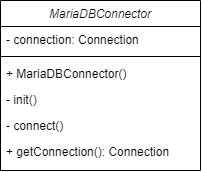
\includegraphics[width=4cm]{MariaDBConnector_before}
        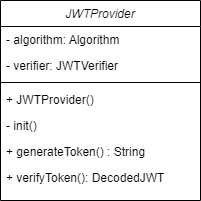
\includegraphics[width=4cm]{JWTProvider_before}
    }
    \caption{\label{1} UML vor Singleton}
\end{figure}

\begin{figure}[htbp]
    \centering
    \fbox{
        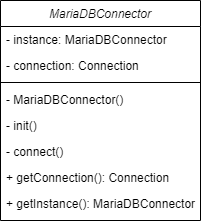
\includegraphics[width=4cm]{MariaDBConnector_after}
        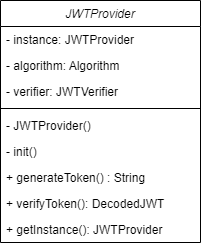
\includegraphics[width=4cm]{JWTProvider_after}
    }
    \caption{\label{2} UML nach Singleton}
\end{figure}


\chapter{Refactoring}

\section{Code Smells identifizieren}

\subsection{1. Long Method APIServer}

\subsubsection{Identifizierung}

Der erste Code Smell den ich im Refactoring fand war der Lange Konstruktor der APIServer Klasse.
Da sollten vor dem Starten des Servers verschiedene Dinge initialisiert und konfiguriert werden.
Da häufte sich aber über die Zeit immer mehr an, was zu diesem Code Smell führte.

\subsubsection{Begründung des Refactorings}

In diesem Refactoring wurde zuerst das Konfigurieren der Kontroller in eine extra Klasse mit dem Namen APIServerConfig ausgelagert.
Diese Klasse wird dann als Parameter des Konstruktors übergeben was es in Zukunft ermöglicht den Server einfacher mit verschiedenen Konfigurationen zu starten.
Danach wurde der AccessManager in die Klasse APIServerAccessManager und die Konfiguration der Endpunkte in die Klasse APIServerEndpointGroup ausgelagert,
wodurch der Code viel verständlicher und überschaubarer wird.
Zuletzt wurde das erstellen der Serverinstanz, für eine bessere Übersichtlichkeit, noch in eine extra Funktion verschoben.
Dadurch wurde der Code insgesammt auf viele kleinere und logische Bausteine verteilt wodurch er einfacher zu verstehen ist.
Zudem konnten durch das aufteilen einfacher sinnvolle Namen für die Methoden der einzelnen Schritte gefunden werden.

\section{Refactorings begründen}
%% 
%% ATRIP - Regeln beim Testen
%% Automatisch 
%% Thorough – Vollständig 
%% Repeatable – Wiederholbar => immer das gleiche Ergebnis liefern 
%% Independent – Unabhängig 
%% Professional – Professionell
%% (Keine unnötigen Tests schreiben, Hilfsfunktionen und Klassen „nur“ zum Testen sinderlaubt und erwünscht)
%% 
%% 
%% 
%% \chapter{Dokumentation}
%% 
%% \section{API}
%% \section{Database}
%% \section{Sonstiges}
\include{8_kapitel}
\pagenumbering{roman}
\setcounter{page}{\thesavepage}
% Ab hier beginnt der Anhang
\appendix
\addcontentsline{toc}{chapter}{Anhang}

\addcontentsline{toc}{chapter}{Index}
\printindex

\addcontentsline{toc}{chapter}{Literaturverzeichnis}

% Haben Sie das "biblatex"-Paket nicht installiert, benutzen Sie folgendes:
% Ohne das "biblatex"-Paket (s. bericht.sty) produziert folgendes
% "deutsche" Zitate in Literaturverzeichnissen gemaß der Norm DIN 1505,
% Teil 2 vom Jan. 1984.
% Die Zitatmarken werden alphabetisch nach Verfassern
% sortiert und sind durch abgekürzte Verfasserbuchstaben plus
% Erscheinungsjahr in eckigen Klammern gekennzeichnet.

% \bibliographystyle{alphadin}
% \bibliography{bericht}

%%%%%%%%%%%%%%%%%%%%%%%%%%%%%%%%%%%%%%%5
% BIBLATEX
% Benutzt man das "biblatex"-Paket, muß man folgendes schreiben:
\def\refname{Literaturverzeichnis}
\printbibliography
%%%%%%%%%%%%%%%%%%%%%%%%%%%%%%%%%%%%%%%5


% 30 mtime=1458147391.399548382
30 atime=1458147391.401548365
30 ctime=1458147391.399548382


% \newpage
% \addcontentsline{toc}{chapter}{Liste der ToDo's}
% \listoftodos[Liste der ToDo's]


\end{document}
